\documentclass[12pt]{scrartcl}
\input{NiaLatexHelpers/nia_defs.tex}
\parskip=0.5cm

\title{\vspace{-2em}Functions and Debugging}
\author{}
\date{}
\begin{document}
\maketitle
\vspace{-6em}
\section*{Programming Functions Are Like Math Functions}
Think of math functions like $f(x) = 3x + 2$ or $f(x) = x^2$. We're often taught to see functions like machines that take inputs and churn out outputs.
\begin{figure}[H]
    \centering
    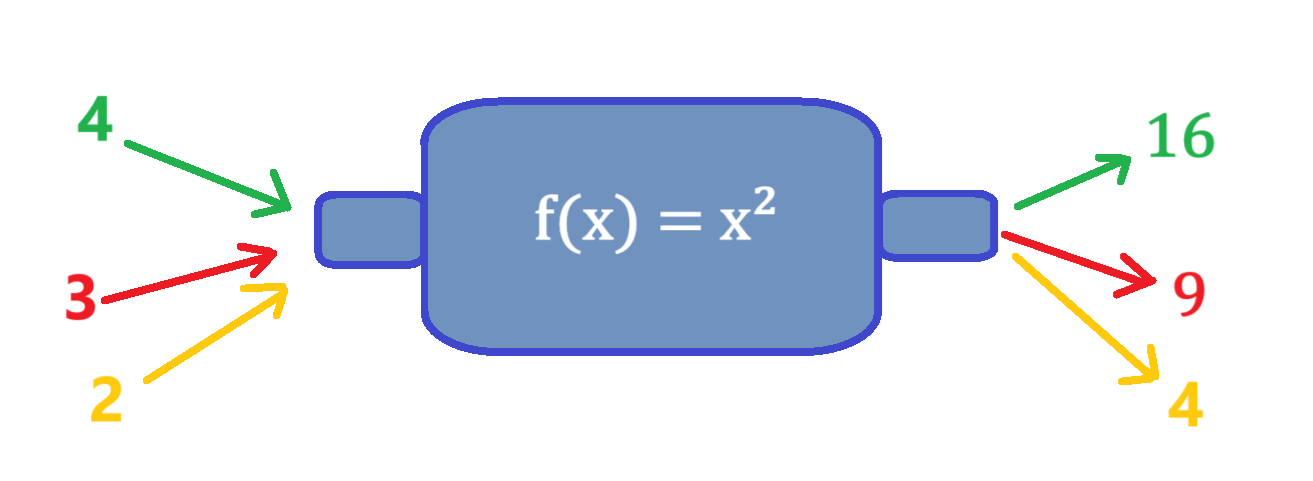
\includegraphics[scale=0.4]{Math Functions as Machines.png}
    \caption*{This function takes in numbers and sqaures them.}
\end{figure}
Programming functions are like that to! Imagine a function that takes in strings (English words) and adds an exclamation point to the end:
\begin{figure}[H]
    \centering
    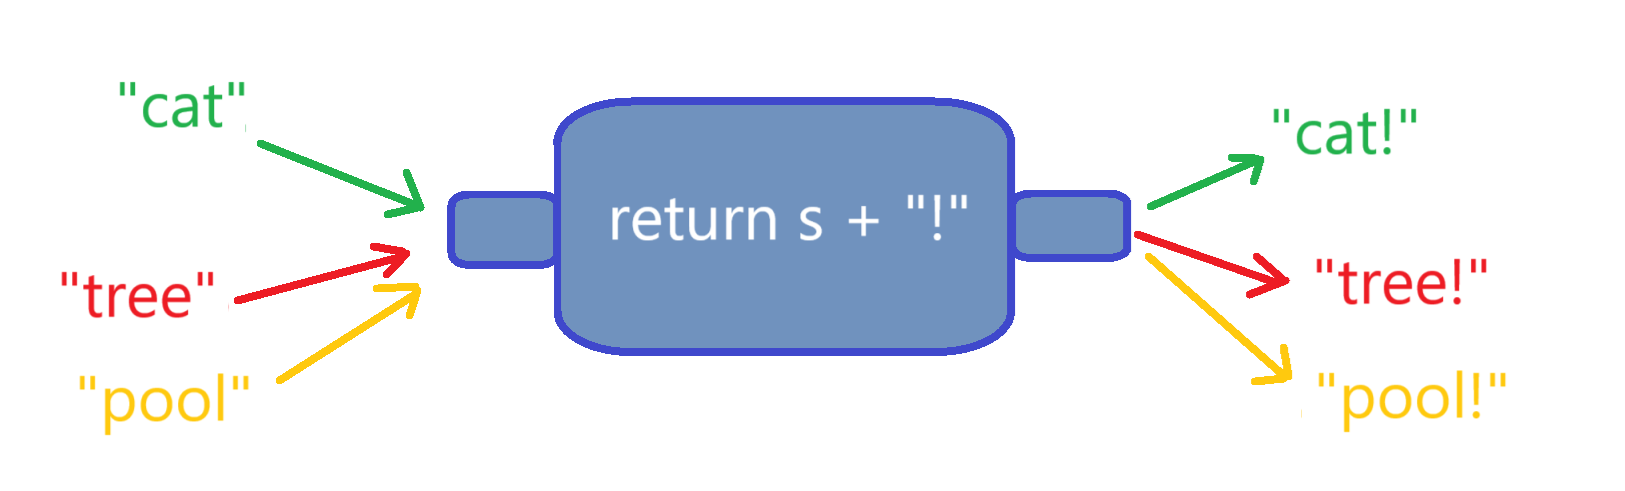
\includegraphics[scale=0.38]{CS Functions as Machines.png}
    \caption*[This function takes in strings and adds an exclamation point to the end.]
\end{figure}
So what would the code be for this function? What's this word \pythonl{return} mean? 

Just like how we can math functions whether we want---$f(x), \: g(x)$, etc---we can call programming functions whatever we want. Let's call this programming function \pythonl{excited} because it takes the English words and makes them look excited. We still don't know what the code is exactly yet for the function, but let's see an example of how the function could be used:
\begin{python}
    message = excited("Welcome")
    print(message)
\end{python}
\begin{code}
    Result: Welcome!
\end{code}
This code sets the variable \pythonl{message} to the result of \pythonl{excited("Welcome")}, which we know will be \pythonl{"Welcome!"}. Afterwards, we get this result and print it to the terminal, so \pythonl{"Welcome!"} will be printed.

Notice how to provide a function input, we use parentheses. In math, if we defined $f(x) = x^2$, then
\vspace{1em}
\[f(2) = 4.\]

It's the same thing here! We put the input in parenthses, so in math notation,
\begin{center}
    \pythonl{excited("cat") = "cat!"}.\footnote{I'm using $=$ here like the math equal sign, not the assignment operator for variables.}
\end{center}
So what's the code for the \pythonl{excited()} function? Here it is!
\begin{python}
    def excited(phrase):
        return phrase + "!"
\end{python}
You start a Python function with the \pythonl{def} keyword. It tells the computer you're creaing a function. Then the input variable is in parentheses. In math, we often have single letter variables like $x$ and $y.$ But in programming, we tend to use variable names with multiple letters so that the code is more easily readable. So think of \pythonl{phrase} as a single input like $x$ and $y$. It's not $p \, h \, r \, a \, s \, e$ as separate inputs; it's only one input!

The colon denotes that we're starting the code for inside the function. Then all the code inside the function needs to be indented. You write \pythonl{return} to say ``This is what the function will spit out.'' We then combined the string \pythonl{phrase} with the string \pythonl{"!"} via the $+$ operator, and we returned/outputted that result!\footnotemark

Notice that even before we knew the code for the \pythonl{excited()} function, we still were able to use the function just fine in the message example from above. This is one of the powers of functions: someone else can write a function, and you don't fully need to understand how that function works in order to be able to use that function. Pretty neat! Functions are a great way to collaborate on coding together.

\newpage
\section*{A Debugging Example}
We did a function that took in strings and added an exclamation point to them. Let's write a function with \pythonl{int}s instead. Let's write the math function $f(x) = 3x + 2$ as code and test it at $x = 5$:
\begin{python}
    def linearEquation(num):
        return 3num + 2

    result = linearEquation(5)
    print(result)
\end{python}
Programming function names can't have spaces, so often we use \texttt{camelCase}, where the first letter of the first word is uncapitalized and the first letter of each subsequent word is capitalized. It's just a naming scheme to help make function names more readable without spaces; you can name your functions whatever you want in Python! Another popular naming scheme is \texttt{snake\_case} where you use underscores.  So the above name would be \texttt{linear\_equation} in snake case.

When we run this function, we get the following error:
\begin{code}
    SyntaxError: invalid decimal literal
\end{code}
What the heck does that mean!? In programming, you'll run into strange errors all the time, and it pays off to become able to research error messages on your own. If you paste this error into a search engine, this \hyperlink{https://stackoverflow.com/questions/59813807/understanding-invalid-decimal-literal}{StackOverflow thread} will come up, a website that will become your friend in due time. If you scroll down, you'll see this comment:
\begin{figure}[H]
    \centering
    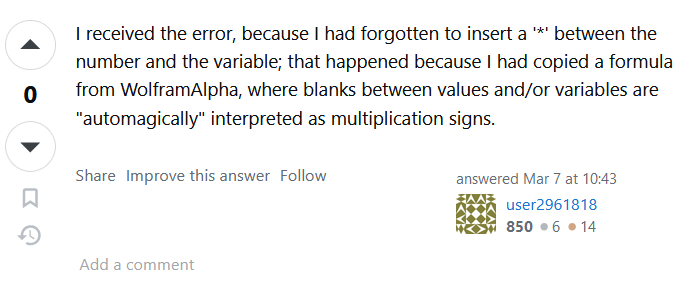
\includegraphics[scale=0.6]{Helpful Message.png}
    \caption*{Oh, thanks random person!}
\end{figure}
The problem was that in Python, mutliplication uses the astrick. We needed to write:
\begin{center}
    \pythonl{return 3 * num + 2}
\end{center}
This is a small little example of debugging, which is fixing a problem in code. Computer bugs are called bugs because once there really was an insect in a computer! This was in 1947 at Harvard University. Nowadays bugs refer to either logical errors (your code does X, but you meant it to do Y) or syntax errors (your code isn't written in a way the computer can understand). Can you guess what kind of bug this multiplication symbol issue was?

It was a syntax error. Syntax errors are recognized by how your computer often can't even run the code at all, while with logic errors, the code can at least run but it gives the wrong output. Logic errors are much more insidious as you can imagine.

We ran into a problem, we researched it, and we found a solution. As we continue our coding journey, we'll learn more tools for debugging.

\newpage
\section*{Functions Allow Easy Code Reuse}
Think of the math function $f(x) = 3x^2 - 3x + 2,$ and imagine we wanted to know all the outputs of this function for $x = 1,\, x = 2,\, x = 3,$ and $x = 4.$ We could write the following Python code:
\begin{python}
    print(3*(1**2) - 3 * 1 + 2) |\qquad In Python, \codel{1**2} means $1^2$|
    print(3*(2**2) - 3 * 2 + 2)
    print(3*(3**2) - 3 * 3 + 2)
    print(3*(4**2) - 3 * 4 + 2)
\end{python}
\begin{code}
    Result:
    2
    8
    20
    38
\end{code}
But that's a lot of writing! Instead, we could write one function and reuse it:
\begin{python}
    def quadratic(num):
        result = 3*(num**2) - 3*num + 2
        return result
    
    print(quadratic(1))
    print(quadratic(2))
    print(quadratic(3))
    print(quadratic(4))
\end{python}
This code has the same output, but we only need to write the complicated math once! And if we change the math, it changes the answer everywhere, which means less chance for us to make typoes. It's a win-win!

Note that we could have just written the function as \pythonl{return 3*(num**2) - 3*num + 2}, but I chose to write the function as two lines just to show that programming functions can be as many lines as we want.

\section*{Functions Can Take in Many Variables}
Our last example today shows another power of functions. Just as you can write math functions with multiple variables (though it's less common to see in high school):
\[f(x,y) = x^2 + y^2,\]
you can write programming functions with multiple inputs. In programming, we call inputs of a function \textit{arguments}. Let's create a function that takes in a string and a number, and for the output it spits out a string with that number of duplicates. See the image below for what I mean:
\begin{figure}[H]
    \centering
    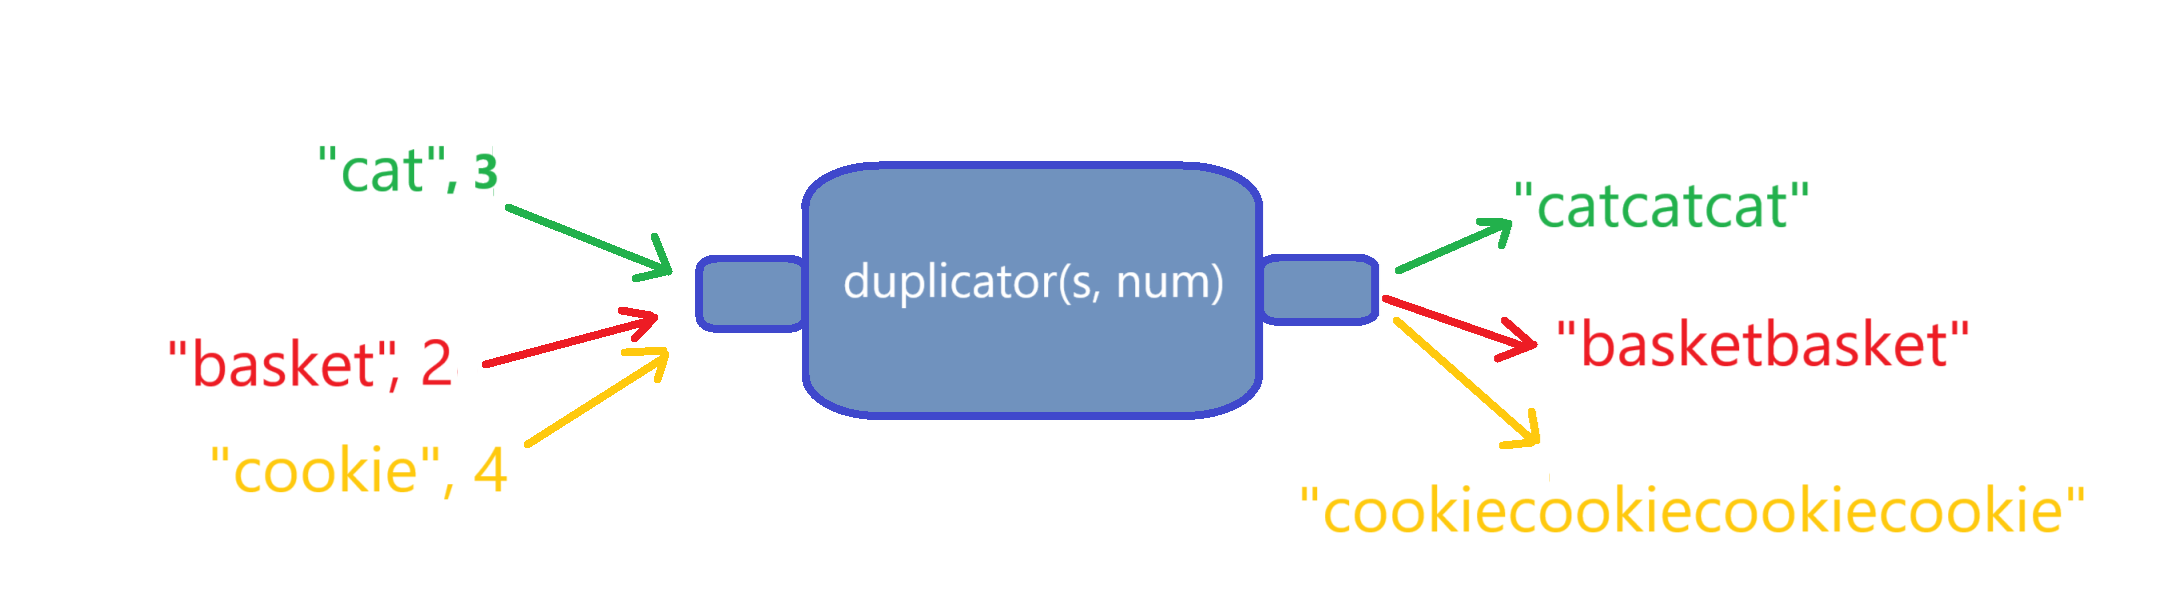
\includegraphics[scale=0.3]{Duplicator Function.png}
\end{figure}
In Python, the \pythonl{*} operator actually lets us do this on strings. Here is the function's code:
\begin{python}
    def duplicator(s, num):
        return s * num
    
    print(duplicator("dog", 5))
\end{python}
\begin{code}
    Result: dogdogdogdogdog
\end{code}
Pretty cool! Most of your functions will have mutliple inputs aka arguments when programming.

\newpage
\section*{Homework}
Attempt the following problems. It's totally okay if you struggle! We'll go over them when we meet again.
\begin{enumerate}
    \item Write a function that takes a string and adds \pythonl{"Happy New Year, "} to the start.
    \item Write a function that gives the negative reciprical of a decimal number (aka a \pythonl{float}). So for example, $3/4$ becomes $-4/3$ and $-2$ becomes $1/2$.
    \item (Challenge) Write a function that takes in two numbers and returns the bigger number. You will have to use an \pythonl{if-else} statement.
\end{enumerate}
\end{document}